\section{Evaluation}\label{sec:eval}

We evaluated the Omni XMP coarray compiler in the environments shown in \tab{specs}.

\begin{table}[bth]
 \caption{Specifications of the computers and evaluation environment}\label{tab:specs}
 \begin{center}\small
  
\begin{tabular}{p{0.09\textwidth}@{~}|@{~}p{0.26\textwidth}@{~}|@{~}p{0.28\textwidth}@{~}|@{~}p{0.30\textwidth}@{~}}
 \hline
 & RIKEN RCCS         & RIKEN RCCS               & CCS, University of Tsukuba \\
 & The K computer     & HOKUSAI GreatWare        & HA-PACS/TCA                \\
 &                    & Fujitsu PRIMEHPC FX100                                \\
 \hline
 \hline
 CPU
 & SPARK64\texttrademark VIIIfx, 2GHz, 128 Gflop/s, 8-core, 1CPU/node
 & SPARK64\texttrademark XIfx, 1.975GHz, 1CPU/node, 4-SIMD $\times$ 32-core
 & E5-2680 v2 (Ivy Bridge), 10-core, 224Gflop/s, 2CPU/node \\
 \hline
 memory
% & {DDR3 SDRAM\\ 128GB/node, 119.4GB/s}   \\
 & 16GB/node,        & 32GB/node,         & 128GB/node,    \\
 & bandwidth 64GB/s  & bandwidth 480GB/s  & 119.4GB/s      \\
 \hline
 inter- connect
 & Tofu
 & Tofu2, 12.5GB/s $\times$ 2
 & InfiniBand FDR, 7GB/s \\
 \hline
 coarray
 & Omni XcalableMP 1.3.1
 & Omni XcalableMP 1.3.1
 & Omni XcalableMP 1.3.1 \\
 \hline
 Fortran
 & Fujitsu Fortran 2.0.0
 & Fujitsu Fortran 2.0.0
 & Intel Fortran 16.0.4 \\
 \hline
 MPI
 & Fujitu MPI 2.0.0
 & Fujitu MPI 2.0.0
 & Intel MPI 5.1.3 \\
 \hline
 comm.\ layer
 & Tofu library
 & Tofu library
 & GASNet 1.24.2 (IBV-conduit, built with Intel compilers) \\
 \hline
\end{tabular}


 \end{center}
\end{table}

%-----------------------------------------------------------------------------
\subsection{Fundamental Performance}
%-----------------------------------------------------------------------------

%===========================================================
%\subsubsection{EPCC Fortran Coarray Micro-benchmark}
%===========================================================

Using the EPCC Fortran Coarray micro-benchmark~\cite{EPCC}, we evaluated the ping-pong performance of PUT and GET communications compared with MPI\_Send/Recv.
The codes are briefly shown in \tab{pingpong-code}.

%-- pingpong-code.pdf
\begin{table}[bht]
  \begin{center}
    \caption{pingpong-code.pdf}\label{tab:pingpong-code}
    % trimはleft bottom right topの順
    \mbox{\includegraphics[trim=24mm 211mm 24mm 16mm, scale=0.7,clip]{figs/pingpong-code-r2.pdf}}
    \begin{flushright}
      {\tt me} is the image index, {\tt id} is the MPI rank number.
    \end{flushright}
  \end{center}
\end{table}
%-- pingpong-fig.pdf
\begin{figure}[bht]
  \begin{center}
    \mbox{\includegraphics[trim=30mm 195mm 32mm 16mm, scale=0.75,clip]{figs/pingpong-fig-r2.pdf}} 
    \caption{pingpong-fig.pdf}\label{fig:pingpong-fig}
  \end{center}
\end{figure}

Corresponding to the codes in \tab{pingpong-code}, \fig{pingpong-fig} shows how data and 
messages are exchanged between two images or processes.
In coarray PUT (a) and GET (b), inter-image synchronization is necessary for each end of 
the phases to make the passive image active and to make the active image passive.
Whereas, in MPI message-passing (c) and (d), such synchronization is not necessary because
both processes are always active.
%
On the other hand, MPI message passing has its own overhead that coarray PUT/GET
does not have. Since the eager protocol (c) does not use RDMA, the receiver
must copy the received data in the local buffer to the target. The larger the data,
the greater the overhead cost.
In the rendezvous protocol (d), negotiations, including remote address notification,
are required prior to communication.
The overhead cost is not negligible when the data is small.


%===========================================================
%\subsubsection{Result of ping-pong benchmark}
%===========================================================

\begin{figure}[p]
  \begin{center}
    % trimはleft bottom right topの順
    %\mbox{\includegraphics[trim=30mm 80mm 30mm 25mm, scale=0.8, clip]{graphs/8graphs-7.pdf}}
    \mbox{\includegraphics[trim=30mm 70mm 30mm 23mm, scale=0.78, clip]{graphs/8graphs-8.pdf}}
    \caption{Ping-pong performance on Fujitsu PRIMEHPC FX100 and HA-PACS/TCA}\label{fig:8graphs}
  \end{center}
\end{figure}
The result of the comparison between coarray PUT/GET and MPI message passing is shown in
\fig{8graphs}.
As the underlying communication libraries, 
FJ-RDMA and MPI-3 are used on FX100 and GASNet and MPI-3 is used on HA-PACS.
GET (a) and GET (b) use the code without and with the optimization described in
\Sec{opt-get}, respectively.
Bandwidth is the communication data size per elapsed time, and
latency is half of the ping-pong elapsed time.
The difference between GET (a) and GET (b) is the compile-time optimization level of the 
coarray translator described in \Sec{opt-get}.


%===========================================================
%\subsubsection{Result of ping-pong benchmark}
%===========================================================

The following was found regarding coarray PUT/GET communication.

\begin{description}

\item [Bandwidth]
Coarray PUT and GET slightly outperforms MPI rendezvous communication for large data 
on FJ-RDMA and MPI-3.
On FJ-RDMA/FX100 (a), the bandwidths of PUT and GET (b) are, respectively, 
+0.1\% to +18\% and -0.4\% to +9.3\% higher than MPI rendezvous in the 
rendezvous range of 32k through 32M bytes.
In addition, on MPI-3 and/or HA-PACS, the bandwidths of PUT and GET are, respectively, +0.3\% to +0.8\% and 
+0.1\% to +1.3\% higher in the rendezvous range of 512k through 32M bytes.
Based on the runtime log, zero-copy communication was confirmed to have been performed
both in PUT and GET (b) by selecting the DMA scheme described in \Sec{opt-dma}.

However, on GASNet/HA-PACS (c), PUT and GET (b) were only approximately 60\% of the bandwidth of MPI rendezvous for a large amount of data.
It is presumed that data copy was caused internally.

\item [Latency]
On FJ-RDMA (a) and MPI-3 (b) and (d), PUT and GET (b) have larger (worse) latency than 
MPI eager communication in the range of $\leq$16kB on FX100 and $\leq$256kB on HA-PACS.

Coarray on GASNet (c) behaves differently than other cases on (a), (b), and (d).
Although the latency is larger than that for MPI for all data sizes, the difference
is smaller than in the other cases. At a data size of 8B, the latency of PUT is 2.93 $\mu$s
and 2.1 times larger than the one of MPI 
while 5.73$\mu$s and 3.7 times larger for the case of MPI-3 (d).

\item [Effect of GET optimization]
For all ranges in all cases, GET (a) has a smaller bandwidth and a larger latency than GET (b).
On FJ-RDMA (a), the bandwidth is 1.41 to 1.85 times improved in the range of 32kB to 32MB
by changing the object code of GET (a) to GET (b).
We found GET (a) caused two extra memory copies. One copy performs the array assignment 
by the Fortran library, and the other copy is from the communication buffer 
to the result variable of the array function {\tt xmpf\_coarray\_get\_generic}. 
The optimization described in \Sec{opt-get} eliminated these two data copies.

\end{description}

The large latency of coarray PUT/GET communication is problematic.
In the next subsection, we discuss how this problem should be solved 
by the compiler and the programming.


%-----------------------------------------------------------------------------
\subsection{Non-blocking Communication}
%-----------------------------------------------------------------------------

For latency hiding, asynchronous and non-blocking features can be expected 
in coarray PUT communication.
The principle is shown in \fig{nonblock-fig}.

%-- nonblock-fig.pdf
\begin{figure}
  \begin{center}
  % trimはleft bottom right topの順
    \mbox{\includegraphics[trim=43mm 144mm 43mm 3mm, scale=0.6,clip]{figs/nonblock-fig-r2.pdf}}
    \caption{Blocking and non-blocking PUT communications}\label{fig:nonblock-fig}
  \end{center}
\end{figure}

\fig{nonblock-fig}(a) shows the half pattern of the ping-pong PUT communication.
Coarray one-sided communication is basically asynchronous, unless 
synchronization is explicitly specified. Therefore, multiple communications
without synchronization, as shown in (b), are closer to actual applications.
In addition, coarray one-sided communication can be optimized using non-blocking communication, as shown in (c).
Blocking and non-blocking communications can be switched with the runtime environment
variable in the current implementation of the Omni compiler.
In MPI message passing, non-blocking communication can be written with 
{\tt MPI\_Isend}, {\tt MPI\_Irecv}, and {\tt MPI\_Wait}.


\fig{8var-pingpong} compares blocking/non-blocking coarray PUT and 
MPI message passing communications.
The two original graphs are the same as those of \fig{8graphs}(a).
Four other graphs display the results of the eight-variable ping-pong program, 
which repeats the ping phase, sending eight individual variables 
from one  to the other in order, and, similarly, the pong phase
in the opposite direction.
Each block size indicates the size of variables, and latency includes the
time for eight variables.

The following was found from the results:
\begin{itemize}
\item
Non-blocking PUT significantly improves the latency of PUT communication. 
From 8B to 8kB, the latency of non-blocking PUT communication is 4.63 times faster on average than blocking PUT. 
Compared to the original PUT, from 8B to 8kB, it performs communication eight times for a period of time 2.11 times longer, on average.
Hiding completion wait behind communication (\fig{nonblock-fig}(c))
greatly improves the performance.

\item
Reduction of synchronization (\fig{nonblock-fig}(b)) itself does not
improve the performance. Compared to the original blocking PUT, 
eight-variable blocking PUT has 9.5 to 10.1 times larger latency for a data set that is eight times
larger.

\item
Unless data size exceeds approximately 8kB, the latency of non-blocking PUT does not
depend on the amount of data. 
The graph of non-blocking PUT is very flat, within $\pm$4\%, over the range 
from 8B to 4kB.

\item 
MPI eager communication has no effect on non-blocking for latency hiding.
The eager protocol, including the unbuffering process of the receiver, appears not to be suitable for
non-buffering.

\item 
Non-blocking coarray PUT outperforms MPI eager message-passing,
except for very fine grain data.
The latency of eight-variable non-blocking PUT is -9\% to 54\% and 18\% to 61\%, as 
compared to eight-variable blocking and non-blocking MPI eager, respectively.
At only two plots for 8B and 16B, the non-blocking PUT is 4\% and 9\% slower 
than the values for blocking MPI. Otherwise, non-blocking PUT is faster than MPI eager, and
the more block size, the larger difference in the latency.

\end{itemize}


\begin{figure}[bth]
  \begin{center}
    %-- 8var-pipo-latency.pdf
    %\mbox{\includegraphics[trim=20mm 52mm 5mm 65mm,scale=0.45,clip]{graphs/8var-latency.pdf}}
    \mbox{\includegraphics[scale=0.45]{graphs/8var-latency-2.pdf}}
    \caption{Eight-variable ping-pong latency on PRIMEHPC FX100}\label{fig:8var-pingpong}
   \end{center}
\end{figure}
    

%\begin{figure}
%  \begin{center}
%    %-- 8var-pipo-bw.pdf
%    \mbox{\includegraphics[trim=40mm 180mm 43mm 0mm, scale=0.6,clip]{figs/8var-pipo-bw.pdf}}\\
%    (a) Bandwidth of blocking and non-blocking communications\\
%    %-- 8var-pipo-latency.pdf
%    \mbox{\includegraphics[trim=40mm 155mm 40mm 0mm, scale=0.6,clip]{figs/8var-pipo-latency.pdf}}\\
%    (b) Latency of blocking and non-blocking communications
%    \caption{8-variable ping-pong on PRIMEHPC FX100}\label{fig:8var-pingpong}
%   \end{center}
%\end{figure}


%-----------------------------------------------------------------------------
\subsection{Application Program}
%-----------------------------------------------------------------------------

The Himeno benchmark is a part of the 2D Poisson equation solver using the Jacobi 
iteration method \cite{himeno}. 
The MPI version of the Himeno benchmark is a strong scaling program distributing
up to three-dimensional nodes. 
%
The K computer shown in \tab{specs} was used in this evaluation.

%===========================================================
\subsubsection{Coarray Version of the Himeno Benchmark}
%===========================================================

For comparison, we prepared the following three versions of Himeno programs.

\begin{description}
\item [MPI/original]
The original MPI version of Himeno benchmark was used as a two-dimensionally 
distributed in the y and z axes. The x axis was automatically SIMD-vectorized 
by the Fortran compiler.
The program executes the computation and communication parts repetitively.
The communication part consists of two steps: z-axis direction communication 
and y-axis direction communication, as shown in \fig{himeno-fig}(a).
Each communication is written with non-blocking MPI message passing and
completion wait at the end of each step.

\item [MPI/non-blocking]
The two-step communication was replaced by non-blocking scrambled communication,
as shown in \fig{himeno-fig}(b).
With this replacement, the number of communications increases from four to eight 
per node, but all communications become independent and can be non-blocking.

\item [Coarray PUT/non-blocking]
The communication pattern is the same as that of MPI/non-blocking.
The data was declared as a coarray, and each communication was written with
a coarray PUT, i.e., an assignment statement with coindexed variable as 
the left-hand side. Since the right-hand side of the statement is a reference
to the same variable as the left-hand side coarray, the PUT communication
was converted to zero-copy DMA-RDMA communication.

\end{description}

\begin{figure}[bth]
 \begin{center}
  \begin{tabular}{c@{~~~}c}
   \mbox{\includegraphics[scale=0.7]{figs/himeno-fig-2step.pdf}} &
   \raisebox{8mm}{\includegraphics[scale=0.7]{figs/himeno-fig-nb.pdf}} \\
   \\
   (a) Original MPI version & (b) Non-blocking MPI and coarray versions
  \end{tabular}   
 \caption{Two algorithms of stencil communication in the Himeno benchmark}\label{fig:himeno-fig}
 \end{center}
\end{figure}

%===========================================================
\subsubsection{Measurement Result}
%===========================================================

\fig{himeno-graph} shows the measurement results for Himeno sizes M, L, and XL,
executed on 1$\times$1, 2$\times$2, 4$\times$4, $\cdots$, 32$\times$32 nodes on the
K computer. The following results were obtained:
\begin{itemize}
\item
PUT non-blocking was the fastest at 76\% of the measurement points of the graph. 
On 1,024 nodes, PUT non-blocking is 1.2\%, 27\%, and 42\% faster than MPI original for sizes M, L, 
and XL, respectively.

\item
As a result of analyzing the contents of elapsed time, it was confirmed that the
difference in the performance is caused by the difference in communication
time. As shown in (b) and (c), the communication times of PUT non-blocking are
56\% and 51\% of those of MPI blocking on 256 nodes on L and XL Himeno sizes, respectively.

\item
MPI non-blocking is not always faster than the MPI original. The effect of 
non-blocking seems to be limited in MPI.

\end{itemize}

%-- himeno-graph.pdf
\begin{figure}[p]
  \begin{center}
    %\mbox{\includegraphics[trim=37mm 34mm 37mm 4mm, scale=0.8,clip]{figs/himeno-graph-r2.pdf}}
    \mbox{\includegraphics[trim=35mm 47mm 30mm 14mm, scale=0.75,clip]{figs/himeno-graph-r7.pdf}}
    \caption{himeno-graph-r2.pdf}\label{fig:himeno-graph}
  \end{center}
\end{figure}


%===========================================================
\subsubsection{Productivity}
%===========================================================

\tab{himeno-lines} compares the scale of the source codes. 
The following features can be found.

\begin{itemize}
\item
PUT blocking requires fewer characters for programming,
especially in subroutines {\tt initcomm} and {\tt initmax}.
The MPI programmer must describe the Cartesian coordinates to represent neighboring nodes in {\tt initcomm}, and must declare MPI vector types to describe the communication pattern in {\tt initmax}. In contrast, the coarray programmer easily represents 
neighboring images with coindex notation, e.g., {\tt [i,j-1,k]}, and 
communication patterns with subarray notations, e.g., {\tt p(1:imax, 1:jmax, 1)}.

\item
The Fortran statement of the MPI program tends to be longer than that of coarray.
Since, comparing PUT non-blocking to MPI non-blocking,
the number of characters is one third while the number of statements is almost the same.
This means that the coarray program is more compact than the MPI program for each
statement. MPI library functions often require long sequences of arguments.

\end{itemize}


\begin{table}
 \caption{Source code scales for the Himeno benchmark}\label{tab:himeno-lines}
 \begin{center}
  
\begin{tabular}{@{~~}l@{~~}*{3}{|r@{~~}r@{~~}r@{~~}}}
 \hline
 subroutine  
 & \multicolumn{3}{c}{MPI original}
 & \multicolumn{3}{|c}{MPI non-blocking}
 & \multicolumn{3}{|c}{PUT non-blocking} \\
 \cline{2-10}
           & LOC   & SOC   & chars  & LOC   & SOC   & chars  & LOC   & SOC   & chars  \\
 \hline
 \hline
 jacobi    & 50    & 33    & 1546   & 50    & 32    & 1546   & 43    & 31    & 1314   \\
 initcomm  & 65    & 39    & 1724   & 80    & 54    & 2380   & 19    & 19    & 421    \\
 initmax   & 95    & 77    & 2336   & 115   & 85    & 2939   & 71    & 71    & 1584   \\
 sendp     & 152   & 59    & 3724   & 299   & 91    & 7617   & 96    & 96    & 2435   \\
 others    & 248   & 225   & 5872   & 250   & 227   & 5923   & 232   & 231   & 5276   \\
 \hline
 TOTAL     &~~~610   &~~~433   &~~15202  &~~~794   &~~~489   &~~29495  &~~~461   &~~~448   &~~11030  \\
 \hline
\end{tabular}
\begin{center}
 \begin{tabular}{l@{~~}l}
LOC:   & Number of lines of codes excluding comment and empty lines. \\
SOC:   & Number of Fortran statements, which may span multiple lines. \\
chars: & Number of characters excluding those in comment lines. \\
 \end{tabular}
\end{center}




 \end{center}
\end{table}

%-- fx100-pipo.pdf
%    \fbox{\includegraphics[trim=4mm 15mm 4mm 3mm, scale=0.9,clip]{figs/fx100-pipo.pdf}}

%himeno.pdf
%latency-16var.pdf
%layer.pdf

%\fbox{\includegraphics[trim=98mm 235mm 98mm 0mm, scale=0.8,clip]{figs/3cell-y.pdf}} \\
%\fbox{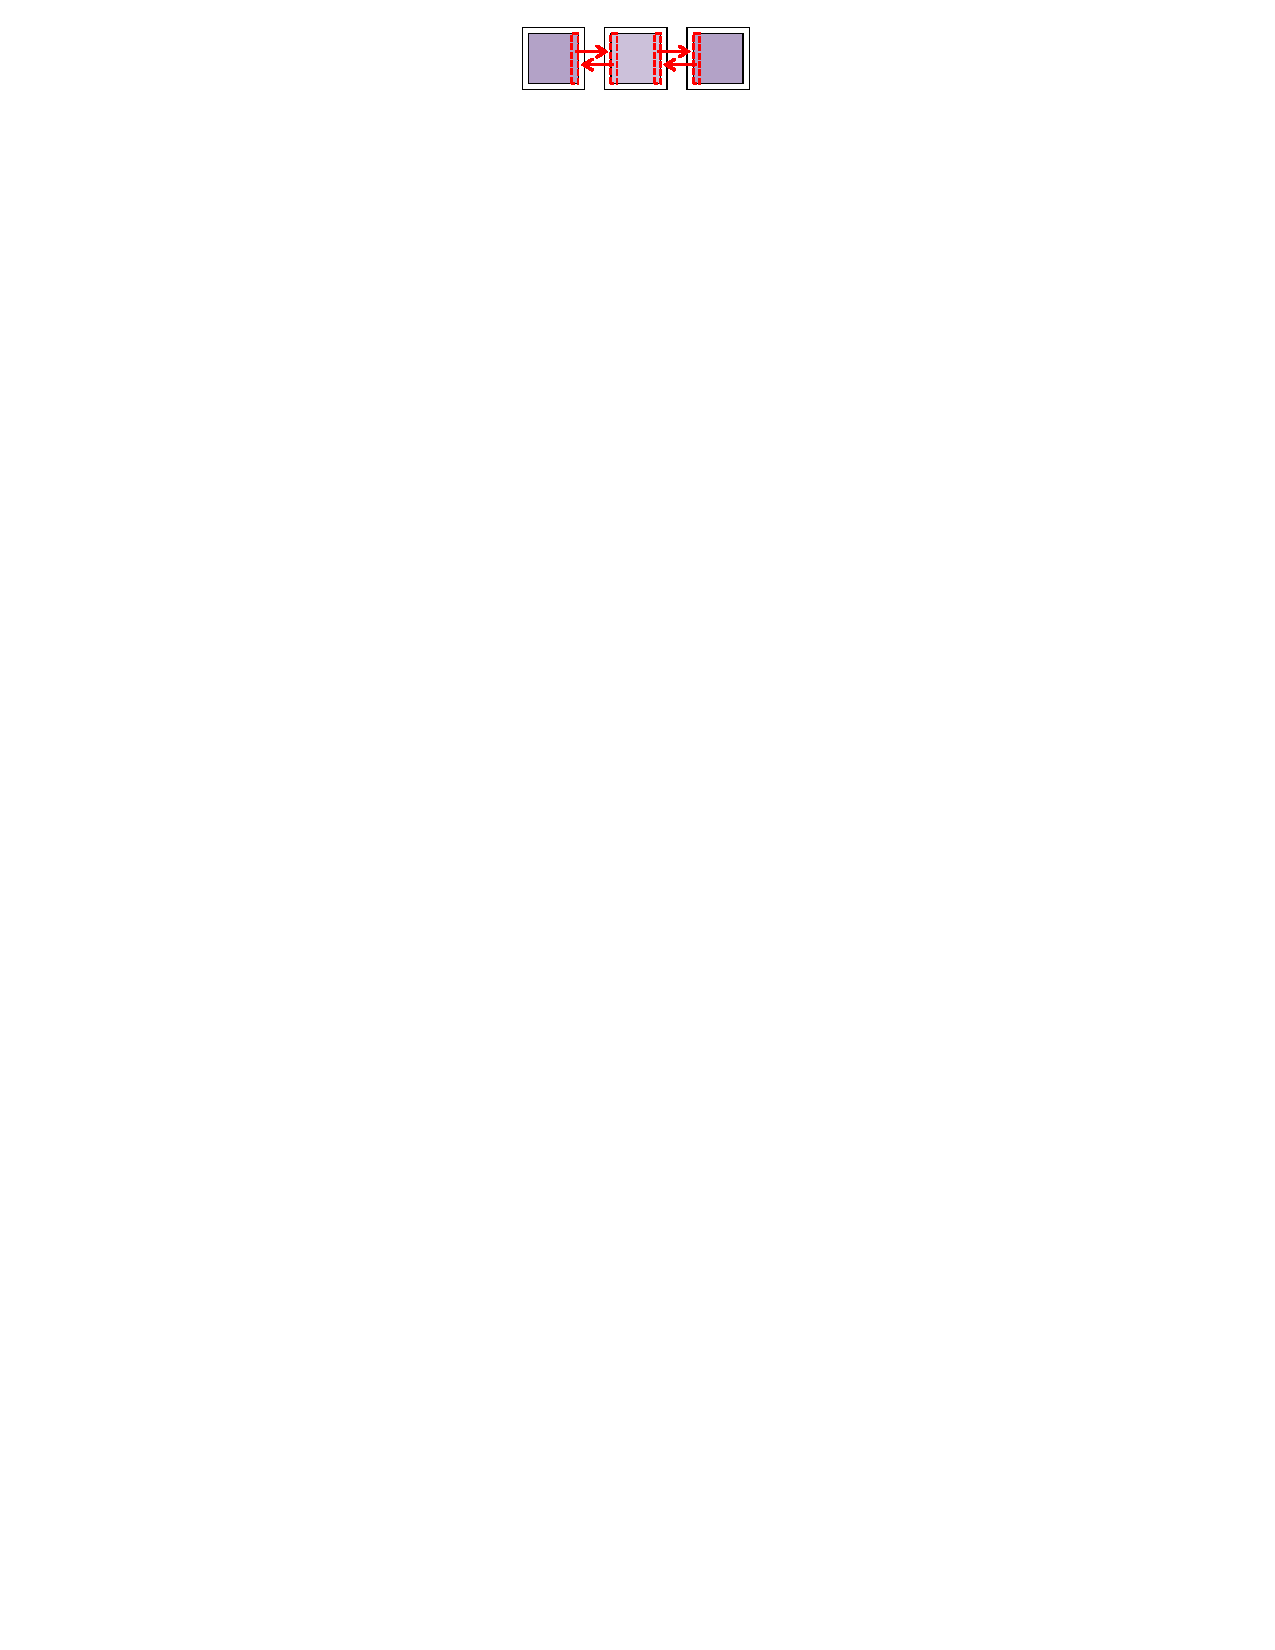
\includegraphics[trim=85mm 261mm 85mm 0mm, scale=0.8,clip]{figs/3cell-z.pdf}}  \\
%\fbox{\includegraphics[trim=82mm 230mm 84mm 0mm, scale=0.8,clip]{figs/9cell-yz.pdf}}

%register-CA-tmp.pdf
%register-RA-CA-tmp.pdf
%register-RA-tmp.pdf
%softstack.pdf
%translator-tmp.pdf



